

\section{Iterations}


\subsection {Testing mobile app technology, conceptual model}
The goal of this iteration was to make a prototype using the proposed technology. The prototype will tell us if it is sensible to use the technology for the project, as well as having a conceptual model to use when discussing initial ideas around the aim of the project, functionality, as well as interaction design.

The technology to be tested was React Native. The reason for this to be the first choice, was to support multiple platforms and not having to rewrite the application for every platform. The same application can be used for Android and iPhone with little modification to the code. React Native is build upon the React front end web development framework, which means some code can be reused for web as well. But all the the views need to be modified, as they use specific React Native components for mobile units. React and React Native are JavaScript frameworks.

We have also used the React web  development framework in previous projects. It s one of the more popular and mature front end web development frameworks in the market. 

The prototype itself and the development process showed that the technology could be used for displaying and organize CPGs. Lessons learned about content flow, databases, app navigation, displaying information and dialogues. JavaScript in the view gives a lot of flexibility compared to just tags.

\begin{figure}[h!]
	\caption {A very simple conceptual model to test one of the proposed technologies, as well as acting as a starting point for discussions}
	\label{fig:ConseptualModel}
	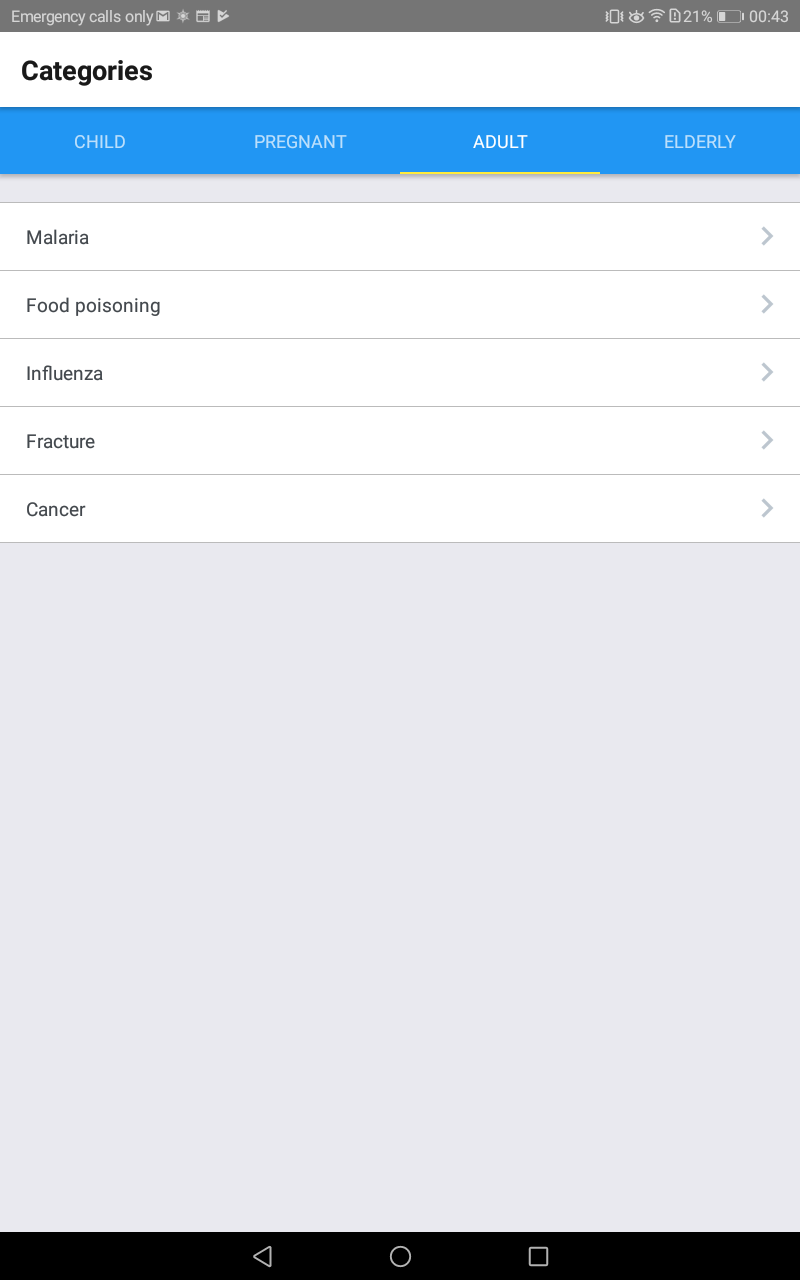
\includegraphics[scale=0.2]{ConceptualPrototype}
\end{figure}

The interface was evaluated with the supervisors, using cognitive walkthroughs. It also worked as a conceptual model, using the prototype as a base for discussing ideas. Both for discussing the purpose of the project, what the user should be able to do, how to organize content and what functionality to add.


\subsection{Studying similar products}
The purpose of the iteration is to see what exists in the market. What have others done. What can we improve, where can we add value to both the medical community and to computer science.

The results from this iteration is presented in appendix \ref{appendix:ComparisonApps}, and was done together with a fellow master of science student in software engineering. As a conclusion, none of these application have a data model which can represent CPGs, nor a patient in a clinical encounter. The representations of CPGs are mostly text based, flow charts or flow charts which expand when you click on decision vertices. LIFE: Neonatal Resuscitation Training is a pretty advanced 3D game, but there is no data model representing the content in the quizzes and tasks.

\subsection{Technology used to represent CPGs}
In this iteration we evaluated technologies which could be used to model CPGs.


\begin{itemize}
	\item \textbf{GLIF} and \textbf{PROforma} was compared during a literature study as a semester assignment in health informatics. We will here give a brief summary of GLIF.
	
	 GLIF or the Guideline Interchange Format, was developed by the InterMed Collaboratory. The intention was to make a guideline representation language, which can be viewed with a various of software application as well as adapting them and making them valid for different local uses. The representation should be precise, ambiguous, readable by humans and interpretable by computers, adaptable to different clinical information standards and facilitating guideline sharing \parencite{Peleg2000}. 

	To make the guidelines readable for humans, interpretable by computers and adaptable by different institutions, GLIF defines the guidelines at three different abstraction levels: conceptual, computable and implementable levels \parencite{DeClercq2008} 
	
	The conceptual level is the highest abstraction level. It consists of
flow-charts which can be viewed by humans, using guideline viewing programs. At this level the guidelines can not
	be used for computations in decision support \parencite{Peleg2000}. 
	
	At the computable level expressions, patient data elements, clinical actions and guideline flow
	are specified at this level. The guidelines can also be verified for logical consistency and completeness \parencite{Peleg2000}.
	
	The implementable level contains the information to incorporate the guidelines into
	the particular institutions knowledge or information system such as EPR \parencite{Peleg2000}.
	
	In figure \ref{fig:GLIFPossibleAsthma} we present a model of the paediatric possible asthma guideline \parencite{RepublicofKeny2016} at the conceptual level. We will now explain the guideline steps the UML-model in figure \ref{fig:GLIFPossibleAsthma} consists of.
	\begin{itemize}
		\item \textbf{Action step} a representation of a recommended tasks or action. There are three types of actions steps: Medically oriented (such as a recommendation for a treatment), programming oriented (such as retrieving information from EHR), control-oriented that invokes nested control structures (subguidelines or macros to support recursive specification) \parencite{DeClercq2008}. Action steps are green squares in figure \ref{fig:GLIFPossibleAsthma}.
		\item \textbf{Decision step} represents a decision point in the model. There are two types of decision steps: Case and Choice. In a Case step the decision will be made up of a number of logical expressions, a deterministic decision. On the other hand, the Choice step displays a various suggestions and the agent (clinician e.g.) needs to choose between them \parencite{DeClercq2008}. Decision steps are turquoise hexagons in figure \ref{fig:GLIFPossibleAsthma}.
		\item \textbf{Patient state step} which characterizes the specific state or condition a patient is in. It can	be used as an entry point into the 
flow-chart, or as an summation to describe the clinical state a patient is in \parencite{Boxwala2004}. Each patient state step includes attributes which describes the condition a patient is in (e.g. iron level in the blood has been reduced since last blood sample). When this condition occurs in practice, the guideline corresponding	to the Patient state step is executed \parencite{DeClercq2008}. Decision steps are yellow diamonds in figure \ref{fig:GLIFPossibleAsthma}.
		\item \textbf{Synchronization step} working together with the \textbf{branch step} to provide multiple concurrency paths \parencite{Boxwala2004}. Multiple guidelines that follows a branch step, eventually comes together in a synchronization step. A continuation attribute specifies	whether all or some conditions need to be fulfilled before we can continue to the next step \parencite{DeClercq2008}. Synchronization and branch steps are not used in figure \ref{fig:GLIFPossibleAsthma}.
	\end{itemize}
	 
	
	\begin{figure}[h!]
		\caption {The paediatric possible asthma guideline \parencite{RepublicofKeny2016} modelled using elements from GLIF}
		\label{fig:GLIFPossibleAsthma}
		\includegraphics[scale=0.132]{GLIFPossibleAsthma}
	\end{figure}
	\item \textbf{Asbru} is another approach for computer interpretable guidelines, and sort of a competitor to GLIF and PROforma. The project was developed at the Stanford University, Vienna University og Technology and Ben-Gurion University. It uses time-oriented skeletal plans. These skeletal plans are schemata at different detail levels. To manage skeletal plans, Asbru introduces some key functionality: the representation of high-level goals (intentions), temporal patterns, time annotations, as well as graphical user interfaces to view the skeletal plans \parencite{DeClercq2008}.
	
	In Asbru, skeletal plans are used to represent guidelines. Each plan's functionality is described by attributes such as: preferences, intentions, conditions, effects and plan body \parencite{DeClercq2008}. 
	
	In figure \ref{fig:AsbruPossibleAsthma}, we have modelled the paediatric possible asthma guideline \parencite{RepublicofKeny2016} using a graphical interface tool AsbruView \parencite{TheAasgardProject2006}. The sequential plans are organized from a start point to an end poing along a time x-axis. Plans can be executed in a parallel, so the y-axis is lanes. Subplans are stacked in z-axis, making the presentation of a guideline 3 dimensionally. In addition to execute plans in sequential or parallel order, we also have the option to execute the in an arbitrary order or without any fixed order (unordered). There are also sequential plans and control structures with if-then-else.
	
	For the skeletal plans shown in figure \ref{fig:AsbruPossibleAsthma}, we can also set the attributes conditions, intentions, effects and preferences for each of them. These describes the functionality of each plan \parencite{DeClercq2008}.
	
		\begin{figure}[h!]
		\caption {An attempt at modelling the paediatric possible asthma guideline \parencite{RepublicofKeny2016}, using Asbru editor tool AsbruView \parencite{TheAasgardProject2006}}
		\label{fig:AsbruPossibleAsthma}
		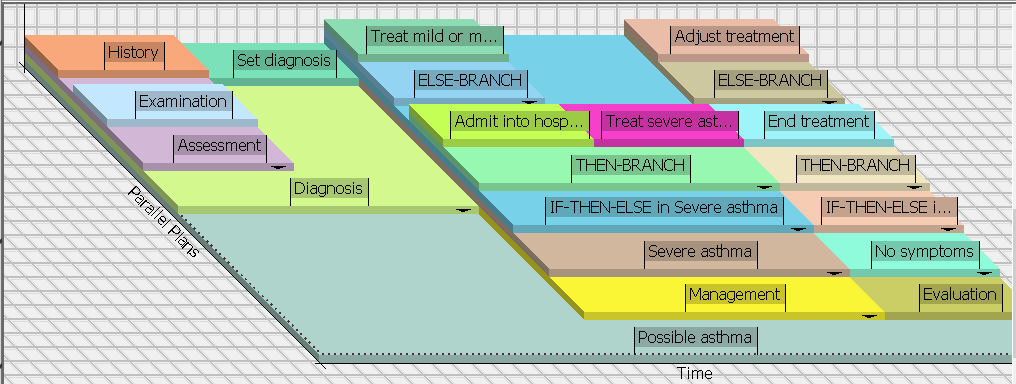
\includegraphics[scale=0.55]{AsbruPossibleAsthma}
	\end{figure}
	\item See the description of \textbf{DPF} in other parts of this thesis.
\end{itemize}
Studying PROforma, GLIF and Asbru we learn that there are several ways to approach the task of making computer interpretable guidelines. We can learn about challenges and see how they solved them. Dissemination, where one needs to regularly update the guidelines and make sure that the different computer systems use the updated versions, is such a topic. Dissemination is relevant for this project, as you want to make sure that every student trains for the most current guideline. You don't want them to memorize old and outdated content.

Our conclusion is that Asbru, GLIF and PROforma are rather large systems, putting a lot of emphasise on working in a hospital setting, communicating with other computer systems such as decision support on the electronic health record. With large computer systems, it is much more difficult to customize.

They also work on a higher abstraction level than the symptoms the clinician needs to look for when doing an examination for asthma. When training clinicians, we are very interested in modeling the details a clinician has to do during a clinical encounter. Asbru, GLIF and PROforma are more concerned with customizing the workflow for one or a sequence of treatments for a medical conditions. We want to use more general models which can be reused to represent several guidelines. With DPF we can create custom domain specific modelling languages.


\subsection{Designing alternatives}
The goal of the iteration is to decide what kind of application to build. What type of application can we best promote the CPGs, and encourage health personnel to use and learn them.

For this iteration it was quite critical to get background information on CPGs, how they are used in the hospital, how they are used by medical students today and how they work in different areas. For this we needed the results from the iterations about the focus group and studying similar products. We also had a medical domain expert in our project. Informal literature studies was also necessary.

A lot of different prototypes at lower and higher fidelities were made. Some were made initially at higher fidelity levels as a part of testing technology. Figure \ref{fig:ConseptualModel} was such a prototype to  test technology, as well as exploring how to organize and categorize CPGs. Figure \ref{fig:SimulationTool} was a prototype of a simulation tool, but also had the purpose of uncovering details of the paediatric possible asthma guideline \parencite{RepublicofKeny2016} when communicating with a medical domain expert. 

Figure \ref{fig:PrototypeInteractiveCPG} was also a prototype initially at higher fidelity as we tested SVG generation with JavaScript. The idea of the prototype was to display CPGs as interactive flow-chart. The vertices have a topic which can be clicked. By clicking, the vertex will either expand to show more detailed information or will redirect to a subguideline. The edges represent decisions and workflow. An idea was also to enter patient specific details such as gender, age and weight and possibly symptoms, and get the CPG customized for that patient.


 \begin{figure}[h!]
 	\caption {A design alternative, displaying the CPGs as interactive flow-charts. The edges represents the flow, while clicking vertices will display more information or redirect to subguideline. A suggestion was to fill in with patient and examination data, to get a customized CPG for a patient }
 	\label{fig:PrototypeInteractiveCPG}
 	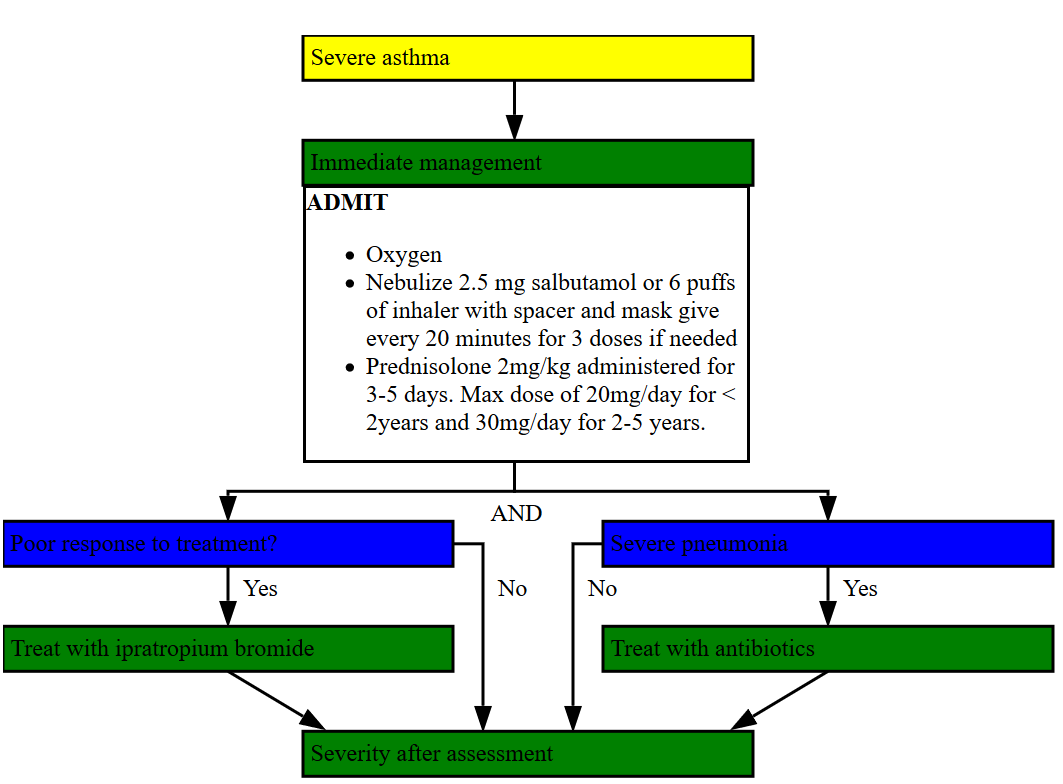
\includegraphics[scale=0.6]{PrototypeInteractiveCPG}
 \end{figure}

The prototype in figure \ref{fig:PrototypeGameCPG}, started as sketches with pen and paper. By going through several iterations of redesign, it reach the fidelity of figure \ref{fig:PrototypeGameCPG}. This was our first prototype where we presented the CPGs as a game. We got help from an external masters degree student in software engineering to make this prototype. The concept of the game is that you initially get presented with a list of tests you can do on the patient. By picking a test, you will immediately get presented with a test result. You can do more tests or proceed. In the next screen you will be presented with a list of treatment and advises, and you should pick the correct ones with the knowledge you acquired in the previous screen. In the last two screens, you will be presented with the answer keys. You will get points for choosing the correct treatments and advises. You will get points for picking the right tests, and you will get higher scores if you picked the tests in an optimal order.
\begin{figure}[h!]
	\caption {The first design alternative proposed as a game. The student tries to pick the right tests in the right order for that patient. As well as choosing the correct treatment and give the right advises to the patient. A high score for choosing the right treatment and advises, as well as correct tests in the right order. Medium score for right tests in the wrong order}
	\label{fig:PrototypeGameCPG}
	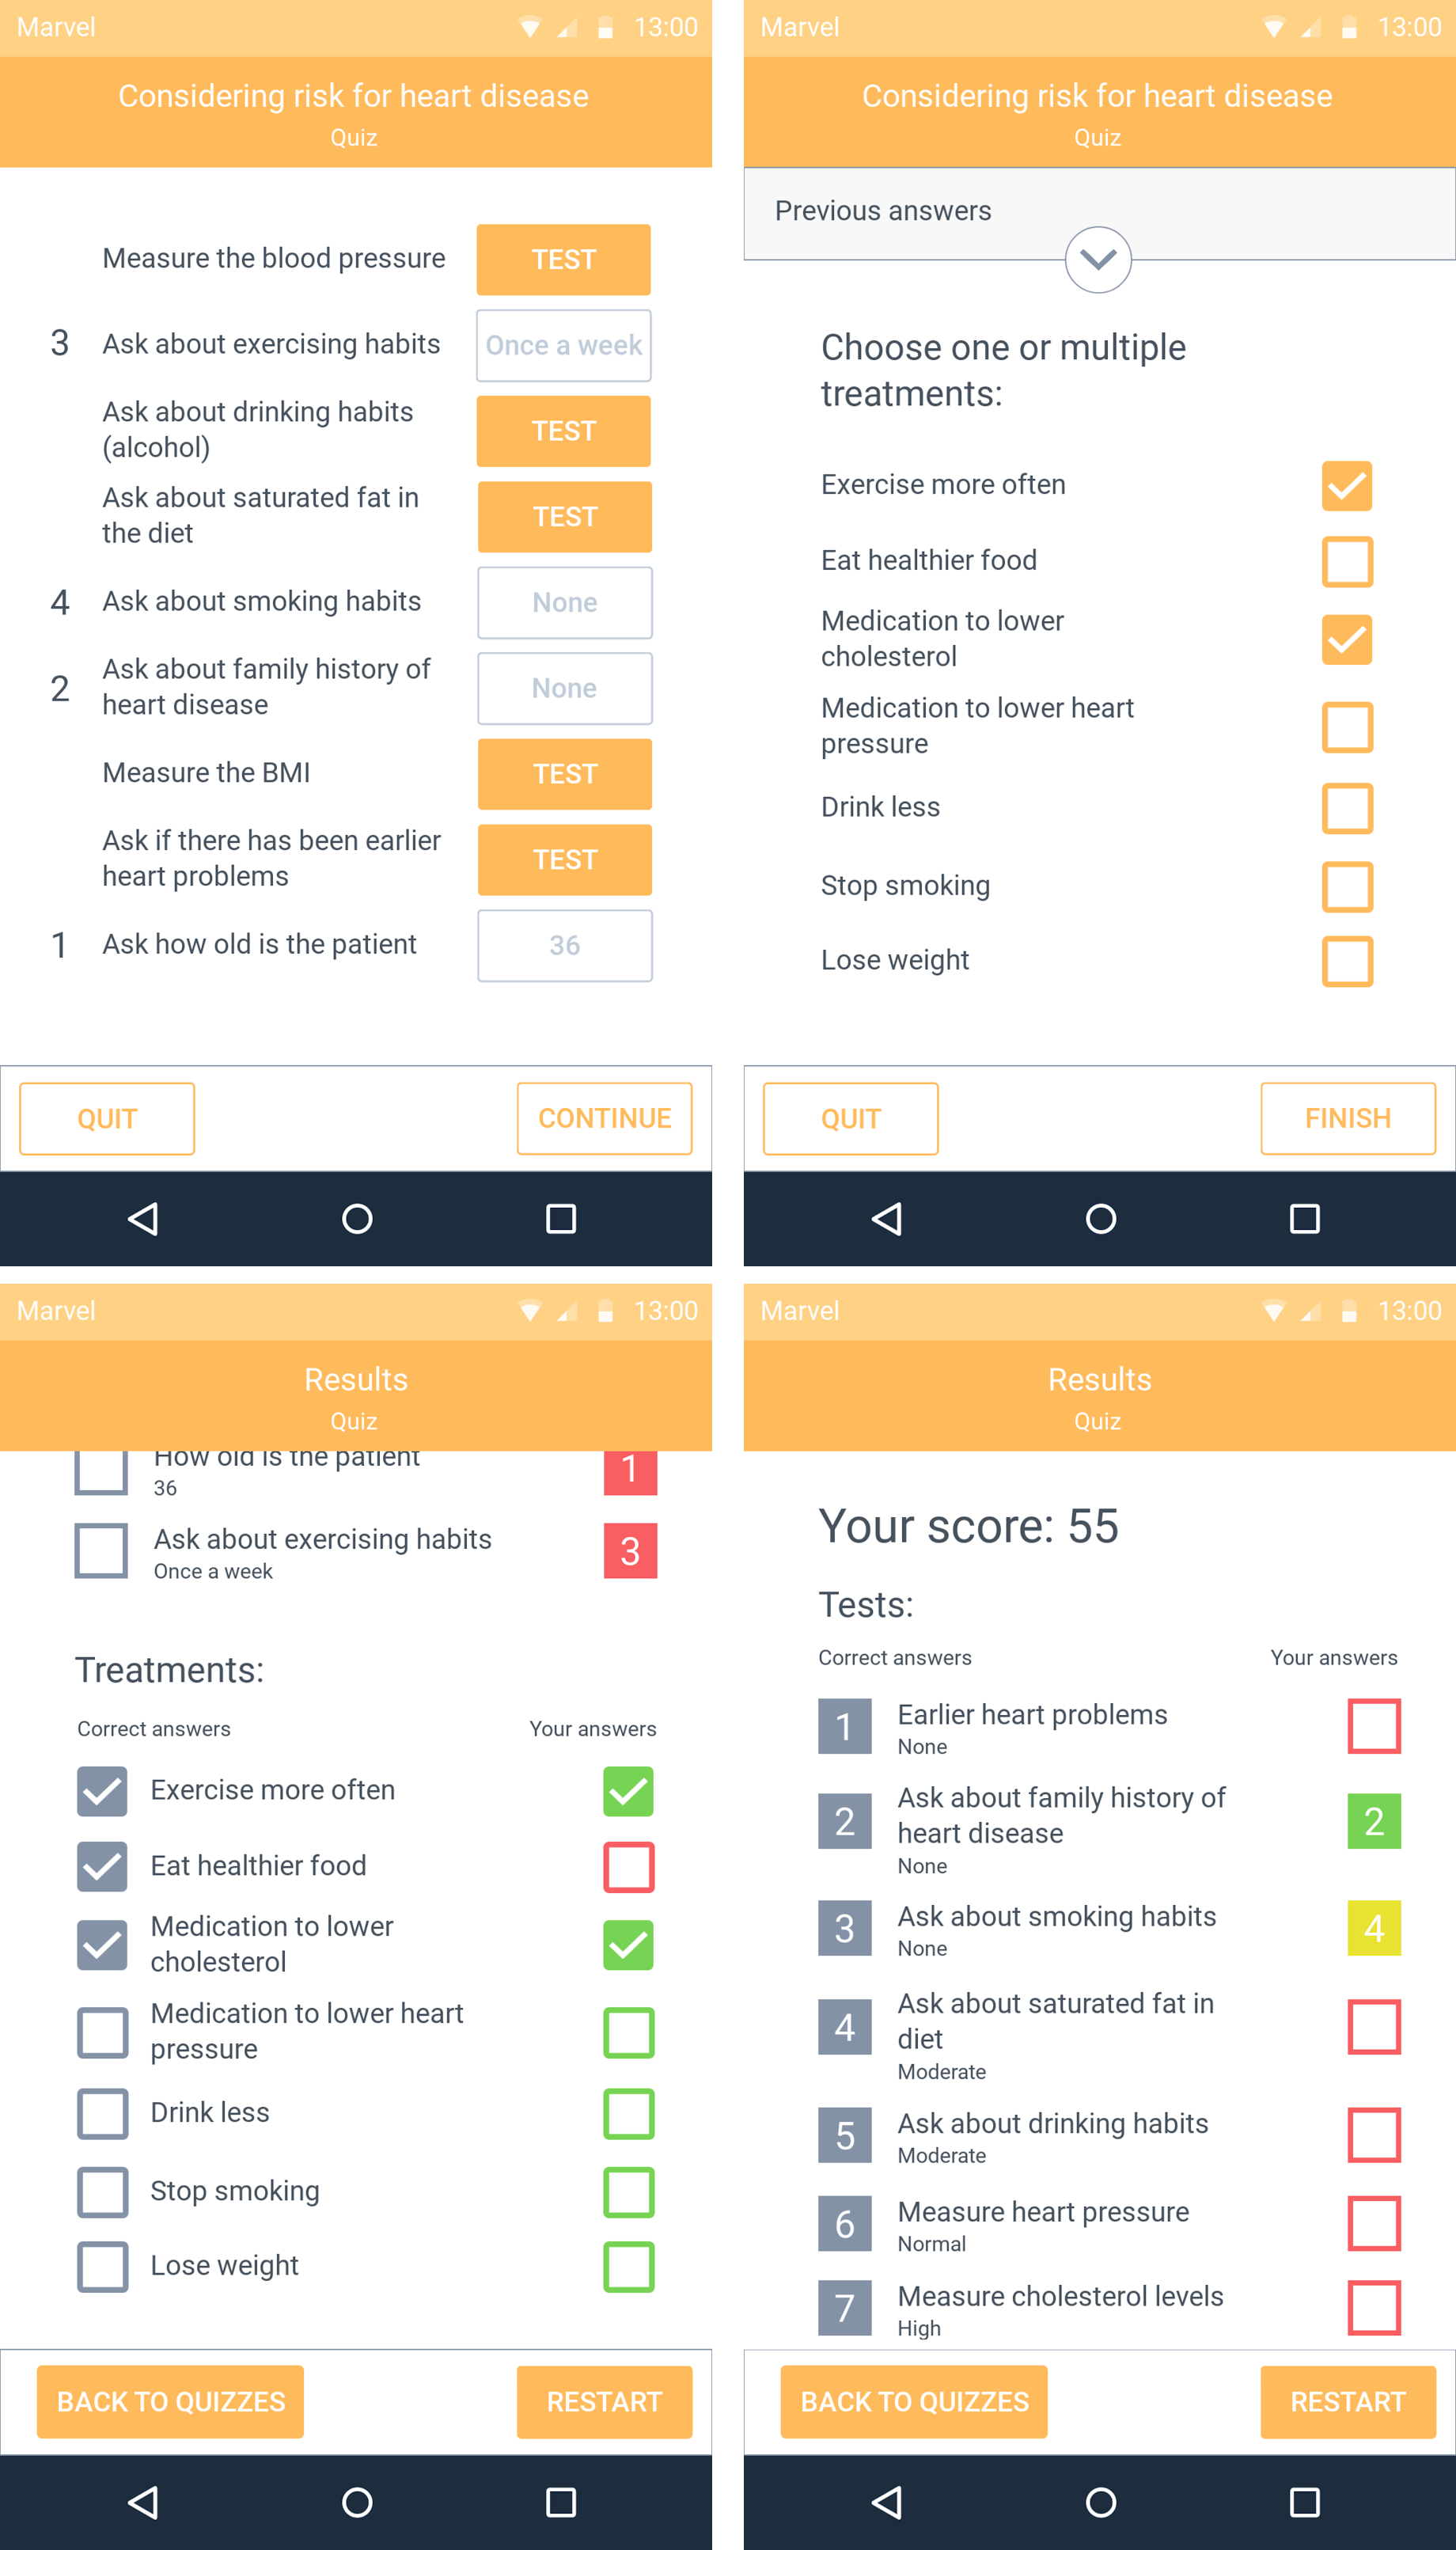
\includegraphics[scale=0.2]{PrototypeGameCPG}
\end{figure}

The design alternatives were evaluated with the project's supervisors and their master degree students. There was also separate evaluations with medical domain expert. The evaluation method was cognitive walkthroughs as well as discussions what is the best approach for promoting CPGs and encourage medical students to learn and use CPGs. The conclusion was to continue with game development. 


\subsection {Entity and workflow models}
The goal of the iteration was to model patients at different stages of the clinical encounter. The entity model should be able to represent patients in scenarios in quizzes with answer keys.

We based our models on the paediatric possible asthma guideline \parencite{RepublicofKeny2016}. The first step was to understand every symptom, medication, equipment used in the treatment and keywords such as "admit". Resources like \textcite{Disease2011} and \textcite{Johansen2018} were some of the resources used, but most importantly was an expert of domain. 

The developer made a prototype of his understanding of the CPG, which simulated a clinical encounter with a patient. See figure \ref{fig:SimulationTool}. The GLIF chart presented in figure \ref{fig:GLIFPossibleAsthma} was used as a base when making the simulation tool. The simulation would start with listing symptoms of asthma and the clinician would choose among the symptoms, redirecting to the treatment for severe, mild, moderate and no asthma. The simulation would continue with cycles of evaluating the given treatment, and the clinician needs to act accordingly to the evaluation for each cycle until the treatment can be ended. An expert of domain got the task of going through the entire simulations of use cases such as "a patient with severe asthma responds poorly to salbutamol treatment". The stimulation gave a thorough understanding of the guideline, emphasized details which would have been missed or details of the treatment which is left out of the guideline itself, such as differential diagnoses.

\begin{figure}[h!]
	\caption {Screenshots of the prototype used to simulate a clinical encounter with a domain expert}
	\label{fig:SimulationTool}
	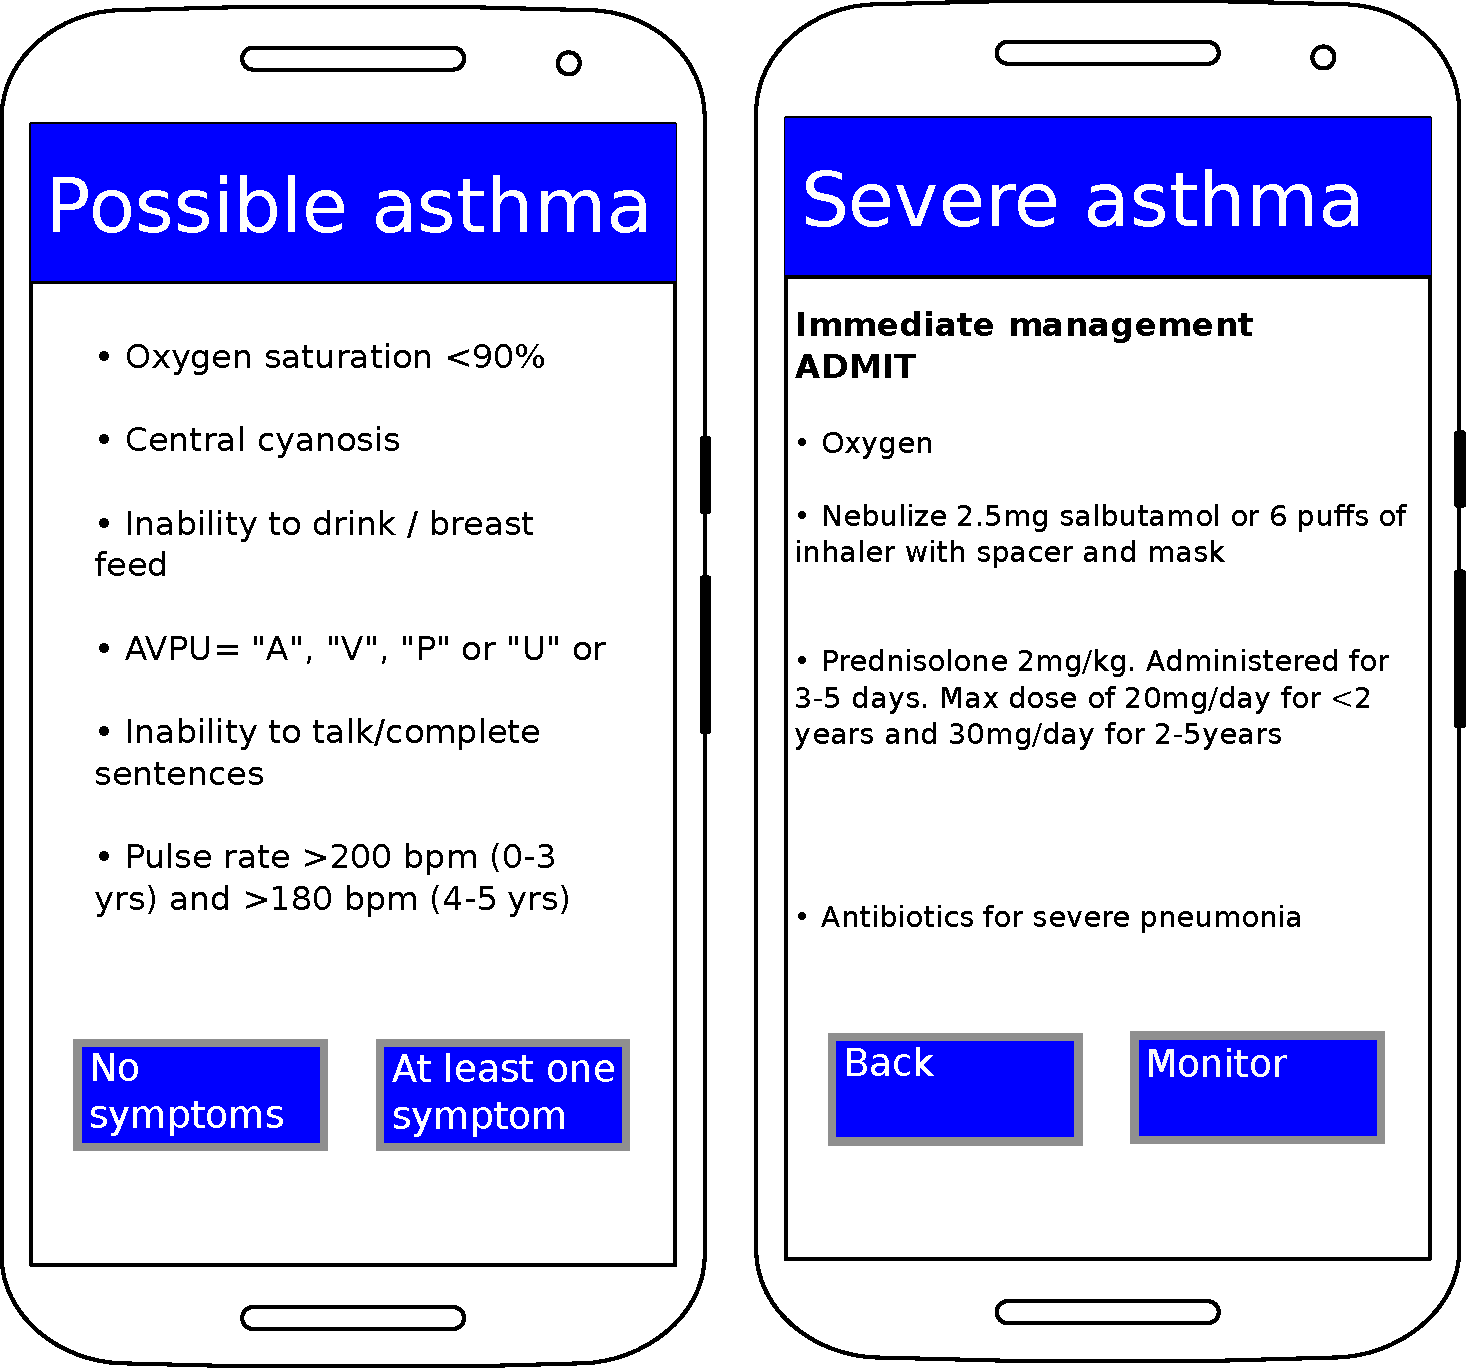
\includegraphics[scale=0.4]{SimulationTool}
\end{figure}

The guideline is also unclear at some points, where a discussion with a domain expert was needed. For example: wheeze + history of cough or difficulty breathing. When parentheses are not used, it is difficult to see if wheeze always needs to be  present, or if it is enough that cough alone is. It is also difficult to understand the effect and model the situation where the presence of a symptom at a certain age gives "increased likelihood" for asthma. In computer science the terms need to be very clear.

A domain expert in Model Driven Engineer and DPF was consulted for discussing problems such as inheritance, how to create good sentences from vertex values in the graph, as well as metamodelling and the use of constraints in DPF. In figure \ref{fig:BlackboardingDPF} there are two images from the whiteboard during the meeting. On the left we see a workflow and an instance below. The XOR is a constraint, which tells that we can choose one of the two  paths only. On te right we see the entity model, and a suggestion with vertices which make good textual presentation of graph values which can be used in texts. 
\begin{figure}[h!]
	\caption {Pictures of the whiteboard during a meeting with domain expert in MDE and DPF. To the left there are some discussion around workflow models. To the right is entity models with vertices which holds a textual representation of the parent vertex.   }
	\label{fig:BlackboardingDPF}
	\includegraphics[scale=0.16]{BlackboardingDPF}
\end{figure}

For evaluating the entity model, a domain expert in medicine made quizzes with factual questions as well as scenario based. By replacing patient related variables in the questions and scenarios, with tags pointing to variables in the entity model, we could see whether the model fulfilled the requirements of displaying good and valid sentences. The sentences were equally good and valid when using different instances of the entity model.

The workflow model got evaluated by making quiz scenarios, and by confirming that these scenarios covered the entire guideline.



 
\subsection{User experience}
The goal of the iteration is to facilitate the application for good user experiences.

First of all we need to clarify what a good user experience is. We are not going to dive in detail into figure \ref{fig:Hassenzahl}, but shortly explain the components he \textcite{Hassenzahl2006} defines.  
\begin{itemize}
	\item Beyond instrumental, has to do with other aspects than reaching a work related goal or solving a work related task. It has to do with attraction and feelings, such as attraction to a beautiful design, the feeling of trust, quality and reliability or the user feels motivated through personal growth and increase of knowledge and skills \parencite{Hassenzahl2006}. 
	\item Emotion and effect, has to do with how the users feel when interacting with the application. Typically we want the user to feel joy and excitement, and damper or prevent feelings such as frustration, anger and disappointment \parencite{Hassenzahl2006}. Typically the user feels satisfaction when completed a work task, or frustrated when the work task takes a long time to complete. 
	\item The experiential emphasizes that the experience is strongly related to the situation it is used in and at which time. \parencite{Hassenzahl2006}. As an example the user experience of listening to your favourite music artist in the car on the way to work, is different from being at a concert in the weekend with the same music artist.
\end{itemize}
\begin{figure}[h!]
	\caption {User experience copied from \textcite{Hassenzahl2006}}
	\label{fig:Hassenzahl}
	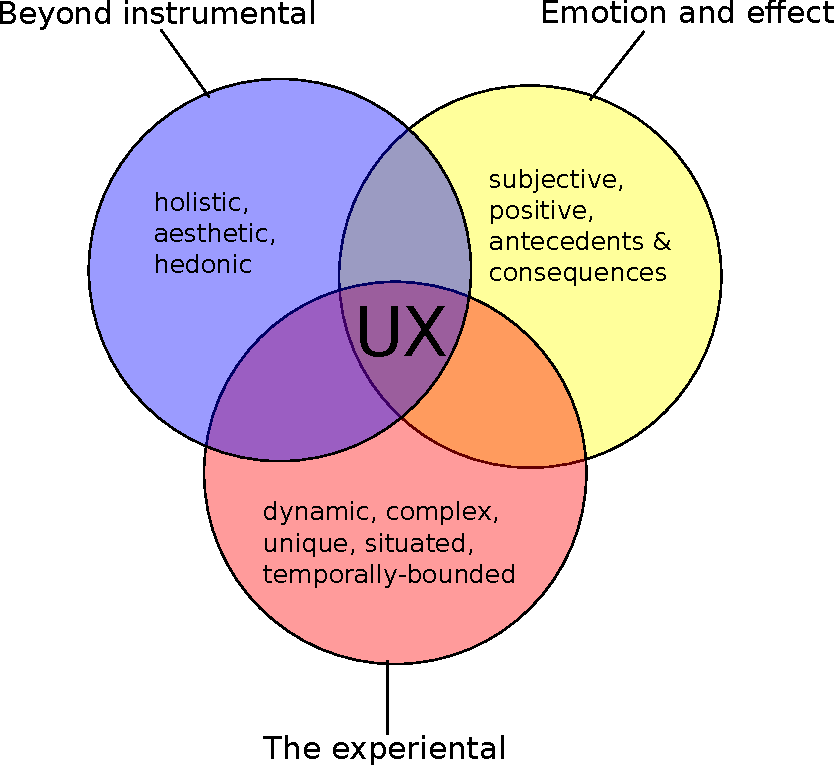
\includegraphics[scale=0.66]{Hassenzahl}
\end{figure}

For the beyond instrumental, we used several iterations to make a pretty user interface to make the application desirable. As this is an educational tool, it is important that the user feels his skills and knowledge grow, so the visualization of progress was quite important. Both that the user advances in levels, but also that we visualize the progress during a level, where the user stretches to slowly meet the requirement of the next level.

For emotion and effect, we should trigger joyful emotions, such as emphasizing when the user answers correctly and progresses. We should use kind and encouraging wording when the user makes an attempt and doesn't get the right answer or doesn't progress to the next level. The interactions should be clear such that the user easily can fulfil his goals and doesn't make mistakes. Keep system errors to a minimal. In our evaluations we could probably more encouraging to the user when he gives a wrong answer.

The experiential use is a bit hard to adapt to. We have been thinking that this is a mobile app, often played when the user is bored and can be situated anywhere. Perhaps on the bus to the university, or waiting for his friends in the cafeteria. The buttons should be large, large font size and small amounts of text on the screen, clear instructions and that the user doesn't have to remember information from previous screens are good guidelines in an environment which can be distracting.

The user experience was evaluated using cognitive walkthroughs with the supervisors and their master degree students. We had a cognitive walkthrough with a domain expert in interaction design and gamification, followed by discussion and tips for further improvement. Some of the feedbacks were "wrong" in red colour may be too harsh, as well as a penalty of negative points even though the penalty is not displayed. A user should be able to get a higher score than just the requirement for the next level.

We used usability tests in controlled environment, where friends, family, fellow students and domain expert in medicine were asked to start the application and play a full quiz. Notes were taken at points where the user would do  mistakes, get confused or do a mistake. Typically the user would become very confused when seeing the screen with the learning map, displaying which levels have been completed, which we are currently playing and the locked levels. The user would typically try to click on completed or current levels. We also noticed that the students wouldn't revise a wrong answer, just continue to the next question.


\subsection{Game Engine}
\subsection{Content flow and creating questions}



\subsection{Focus group}

\subsection{Workshop}